% Activate the following line by filling in the right side. If for example the name of the root file is Main.tex, write
% "...root = Main.tex" if the chapter file is in the same directory, and "...root = ../Main.tex" if the chapter is in a subdirectory.
 
%!TEX root =  

\chapter{Design}
\label{design}

\minitoc

This chapter describes the design phase of the program, where the program architecture is established. Several critical decisions are made in this phase and the design and architecture decisions impacts the way the implementation phase proceeds as it defines how the final software system is decomposed into modules, and how these modules behave and interact with each other. 

In implementing Privacy Advisor, a class structure is built around the CBR agent model discussed in the paper by T{\o}ndel and Nyre. Given the broad structure in the CBR agent model, several details need to be fleshed out, including data structures for storing policies, databases, choosing actual algorithms, a user interface, and so forth. This chapter lays out the broad structure of the Privacy Advisor system. Implementation details are discussed in Chapter~\ref{Implementation}.

%%
%% This chapter should be organized as follows: 
%% - overview
%% - io/gui/cli
%% - cbr engine
%% - data objects storage


\begin{figure}[htbp]
\begin{center}
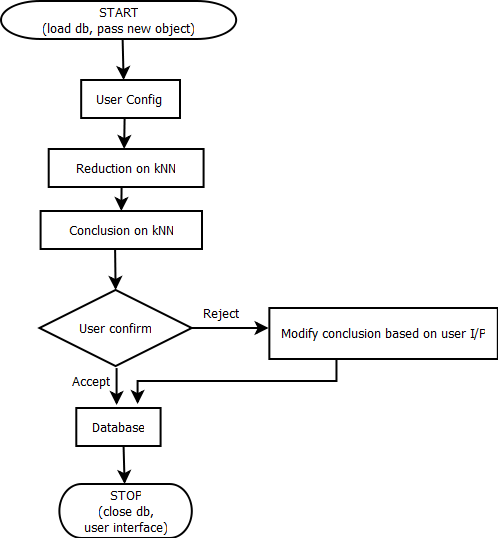
\includegraphics[width = \textwidth]{DesignReport/uml/flowchart.png}
\caption{Program Flow.}
\label{DesignFlowChrt}
\end{center}
\end{figure}

\section{Design Overview}
This section describes the architecture of the local CBR based system. The next section gives an overview over the design of the server component using collaborative filtering and how it interfaces with the local system.  

\begin{figure}[htbp]
\begin{center}
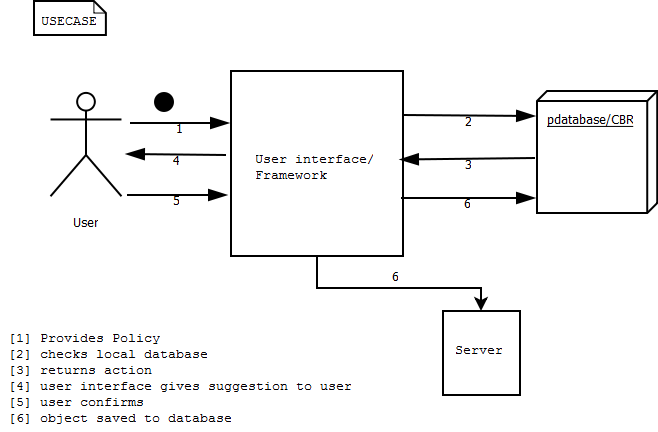
\includegraphics[width = \textwidth]{DesignReport/uml/Case.png}
\caption{System Overview.}
\label{SystemOverview}
\end{center}
\end{figure}

\subsection{Program Flow}
Figures~\ref{DesignFlowChart} and \ref{SystemOverview} seek to provide a broad overview of the structure of the Privacy Advisor system. The program flow is given by Figure~\ref{DesignFlowChart}: a policy object is passed to the CBR system from the user, either through the CLI or GUI. The CBR does a lookup on similar cases in the local database and computes an initial recommendation based on the similar cases retrieved. If the confidence in this recommendation is above a given threshold, it provides the user with the advice and the background for the advice through the user interface. If the confidence is not sufficient, the system will query the community system for an advice, which then is combined with the initial recommendation for a final advice which is presented to the user. The user can then give a feedback on the advice choosing to accept or reject it. The user feedback is then stored back to the database.



\begin{figure}[htbp]
\begin{center}
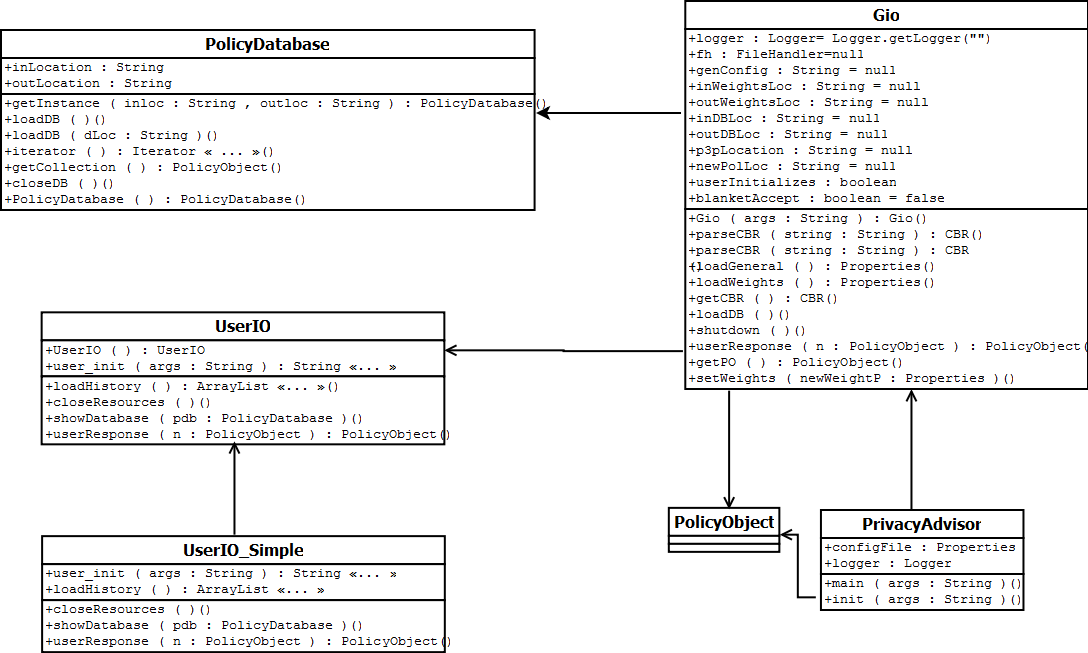
\includegraphics[width = \textwidth]{DesignReport/uml/gio.png}
\caption{Input/output and user interfaces.}
\label{UserIO}
\end{center}
\end{figure}


\section{User Interfaces and Input/Output}
Privacy Advisor can be run using either a command line interface (CLI) or a graphical user interface (GUI). Both the CLI and the GUI are built on top of a "General Input/Output'' module, GIO. GIO creates the database objects and issues the proper commands to the CBR framework based on user input. The GIO class is shown in Figure~\ref{gioFig}. 

\begin{figure}[htbp]
\begin{center}
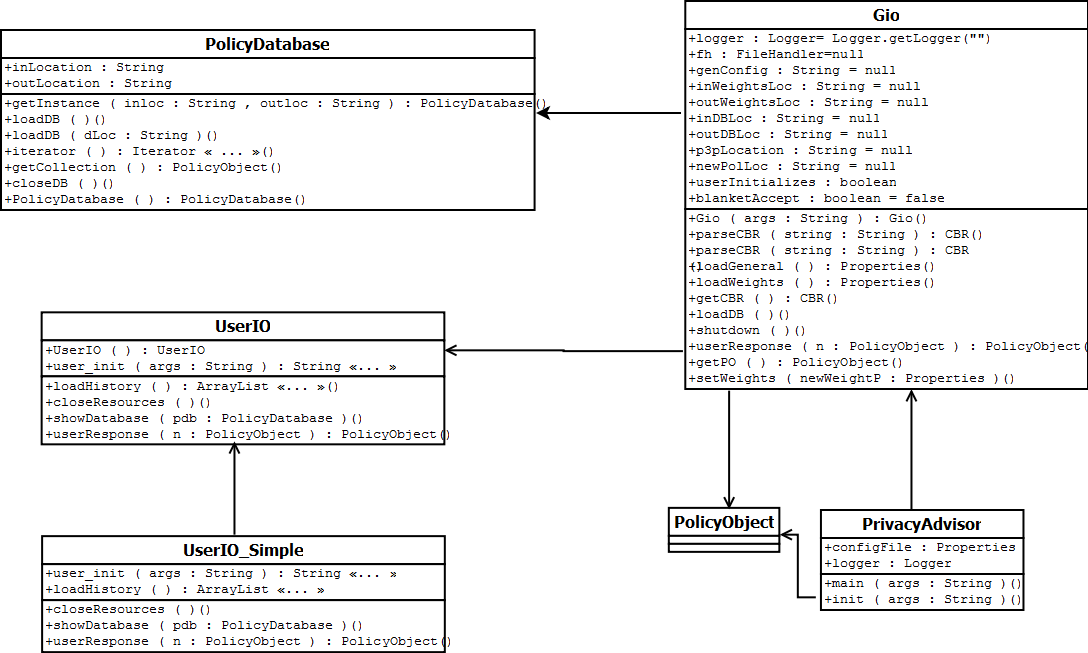
\includegraphics[width = \textwidth]{DesignReport/uml/gio.png}
\caption{working of system.}
\label{gioFig}
\end{center}
\end{figure}


\subsubsection{Graphical User Interface} 
%TODO Einar

\begin{figure}[htbp]
\begin{center}
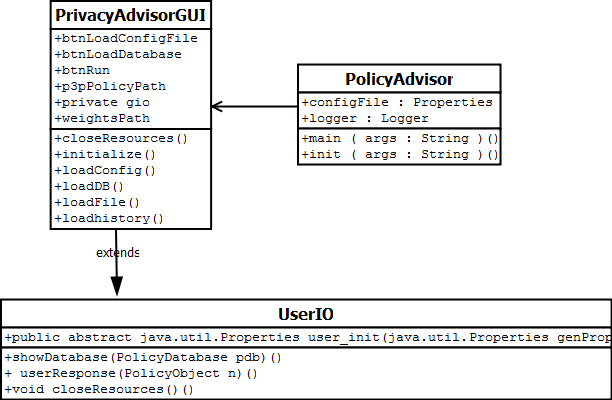
\includegraphics[width = \textwidth]{DesignReport/uml/policyadvisorgui}
\caption{GUI interfaces.}
\label{GUI_interface}
\end{center}
\end{figure}

\subsubsection{Weights and Configuration Files}
As an addition to passing command line arguments, GIO also reads a text based configuration file containing CBR and database settings. The configuration files are detailed in the User Documentation in table~\ref{configTable}. 

\subsubsection{CBR} % TODO Nicholas: Why PDatabase is not connected directly to CBR
Input from the UI is passed on to the CBR framework. CBR in turn references three other key modules, a \emph{reduction} algorithm, a \emph{conclusion} algorithm, and finally, a \emph{learning} algorithm.

The reduction algorithm searches the database to find the most similar cases to the new case presented. The canonical reduction algorithm is k Nearest Neighbors, discussed in section~\ref{kNN}. The conclusion algorithm looks at the set of cases returned by the reduction, and decides on the most appropriate action for the novel case. It also returns a measure of confidence in the conclusion reached.

Finally, a learning algorithm allows for automatically tuning the parameters used for distance calculations. This is discussed further in section~\ref{learnAlgos}.

An overview of the CBR system is given in Figure~\ref{cbr_fig}...
% comment reduction, learning, conclusion, KNN


\begin{figure}[htbp]
\begin{center}
\includegraphics[width = \textwidth]{DesignReport/uml/CBR.png}
\caption{CBR System.}
\label{cbr_fig}
\end{center}
\end{figure}




\section{Data Objects and Storage}

\subsection{P3P Policy Objects}\label{p3pPolObj}
An overview of the Policy Object is given in Figure~\ref{po_fig}...

A P3P Policy Object consists of an \texttt{Action}, a \texttt{Context} and a list of different \texttt{Case} objects. The action object consists of the result from the comparison algorithm, stating if the policy is accepted as a good match, the reasons for this statement and with how much confidence this statement is correct.

The context objects holds most of the objects context, that is what domain the policy belongs to as well as when it was created, last accessed and when it will expire. The list of cases contains one case for each datatype within the policy. A datatype is what kind of information is collected, for example name or date of birth. Each case contains what the purpose for this information is, who are the recipients and the retention for this information. Each datatype has its own case as it simplified the comparison algorithm.

The last thing a policy object contains is a hashmap of the entity data. This is the data that is included at the beginning of every policy document and contains information about the company in question.

\begin{figure}[htbp]
\begin{center}
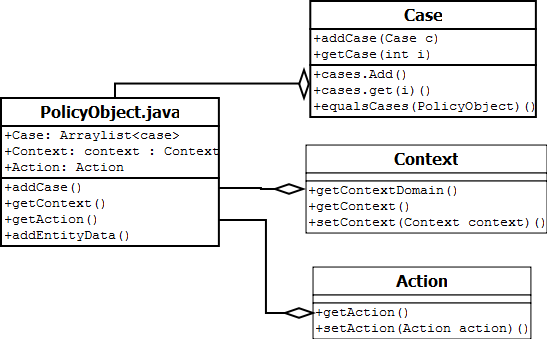
\includegraphics[width = \textwidth]{DesignReport/uml/po.png}
\caption{Policy Object.}
\label{po_fig}
\end{center}
\end{figure}

\subsection{P3P Policy Database}

An overview of the Policy Database is given in Figure~\ref{pd_fig}...

The local case history, maintained in a local database, is stored via a concrete class implementing 'PolicyDatabase'. This abstract class details the required methods for a local policy database: a singleton constructor for the database object; a call to load the database once constructed, from disk; a method adding a single policy to the database; a method returning a Java iterator over the stored PolicyObjects, and a call to return all policies from a given domain.

In order to ensure consistency, the local policy database enforces singletonness. The database object itself is constructed without the actual history, requiring a seperate parameter-less 'loadDB' call on it to load policies from disk to the class, if necessary.

During the CBR cycle, it becomes necessary to check past cases for relevancy during the 'retrieve' phase. This is accomplished by using the standard java Iterator return by \texttt{getiterator()}.
Finally, the CBR cycle concludes by saving the new case (using 'addpolicy(newpolicy)'), and closing the database using 'closeDB()' (which is when the cases would be saved to disk).

An overview of the Policy Database is given in Figure~\ref{pd_fig}...



\begin{figure}[htbp]
\begin{center}
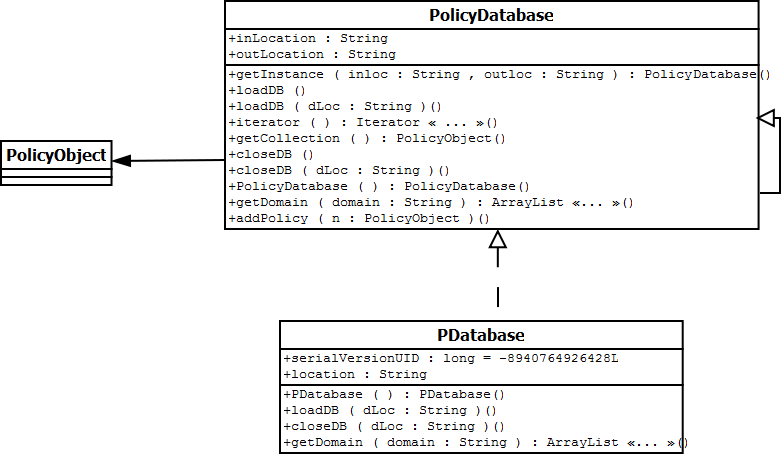
\includegraphics[width = \textwidth]{DesignReport/uml/pd.png}
\caption{Policy Database.}
\label{pd_fig}
\end{center}
\end{figure}

\subsection{Interfaces}







\subsection{Community Server} %%TODO needs rewrite- focuse here is on design not implementation. mention query should be server-side
The community knowledge repository is implemented using a public CouchDB (no-SQL server), which is accessed using standard Java to JSON java libraries. The client program (end-user java application) communicates with the server at two points- when the application has insufficient knowledge, or confidence in its knowledge, to make a suggestion as to the acceptance of a new P3P policy; and after the user has confirmed or overridden the policy.

In the first instance, the new policy under consideration is converted to JSON using GSON (the Google Json libraries), and transmitted to the database, which parses the new policy and replies with a JSON encoded suggested Action.

In the second instance, the final policy (including the action taken on it) is sent to the CouchDB server, and the server proceeds to store the object.
On the database end, there are two essential interfaces (beyond any standard initialization and shutdown procedures). As seem above, these two interfaces are the suggestion provider, which includes a query to find the most similar policies and actions on them by the community, and a interface to simply save the new policy to the appropriate database.
The database is easily replaceable, requiring only the construction of a new class implementing 'NetworkR', the abstract class detailing the methods called by the PrivacyAdvisor framework. The selection between available 'NetworkR' implementations in made by setting the 'NetworkRType' configuration variable during initialization to the full classname.
